\documentclass[a4paper,10pt]{article}
\usepackage[utf8]{inputenc}

\usepackage{cite}
%\usepackage{natbib}

\usepackage[hyphens]{url}
\usepackage[hidelinks]{hyperref}
\hypersetup{breaklinks=true}
\urlstyle{same}

\usepackage{graphicx}
\usepackage{float}

%opening
\title{}
\author{}

\begin{document}

\maketitle

\begin{abstract}

\end{abstract}

\section{Conclusiones de artículos leidos e ideas a implementar}

\subsection{Estrategia para la selección del dataset y su procesado}

The COVID-19 Open Research Dataset (CORD-19) presented by \cite{CORD19} has been used. CORD-19 contains a mixture of articles and preprints on COVID-19 and similar past coronaviruses like SARS and MERS. This resource was developed as an initiative to bring together the machine learning community with experts in the biomedical domain to identify effective treatments and management policies for COVID19. The CORD19 release used was the June 2, 2022 release. This version contains 401,214 documents from different years; the distribution of articles by year can be seen in Figure \ref{fig:Histogram_Available_Papers_Year}.

\begin{figure}[H]
    \centering
    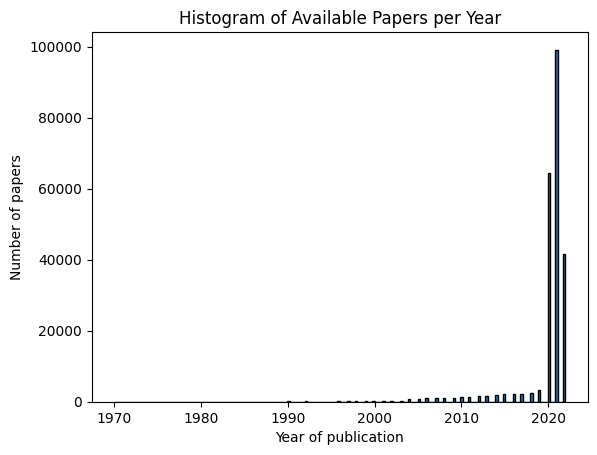
\includegraphics[width=0.8\linewidth]{fig/Histogram_Available_Papers_Year.png}
    \caption{\centering Distribution of papers in the corpus according to their publication date.}
    \label{fig:Histogram_Available_Papers_Year}
\end{figure}


The information available for each article is as follows: title, authors, abstract, text, bibliographic entries, internal references (tables, figures or elements within the article with their respective title) and acknowledgements. In addition to this information, the following metadata is also available for each paper: the source from which it originates, its doi, the license of use, its date of publication and the journal in which was published.

Data preprocessing is one of the most critical processes when generating topic models. Is important to remove as much noise as possible while keeping the relevant terms. The more words that are removed, the faster, more efficient and more correct the models will be. For this reason, inspired by the guidelines given by \cite{LDAMethodology}, these steps have been followed for the text preprocessing:

\begin{enumerate}
    \item Due to the available resources and the large number of articles, it has been decided to work only with the abstracts of the articles. In this way, the computational cost of this phase was reduced. Considering the small number of articles that did not have abstracts, it was decided to discard them and not take them into account. In addition, there are papers in the corpus with publication dates later than the corpus version. Given the distortion that these articles can generate in the models, it has been decided not to take them into account. Thus, only previously published articles are used.

    \item The corpus contains articles in several languages. The main language is English, so it was decided to filter the articles to use only those written in English. The \textit{Langdetect} package was used to identify the language of the texts.

    \item The text has been lowercased in order to group terms by character and not by their format. Observing the content of the abstracts, some DOI links have been found, therefore, and before carrying out the following steps, all the links have been deleted.

    \item All stopwords present in the texts have been removed. The list of stopwords has been extracted from the repository \textit{stopwords-iso}\footnote{https://github.com/stopwords-iso/stopwords-iso}. In this repository, stopwords from different sources have been collected in order to create a list as extensive as possible.

    \item Punctuation characters and all numbers have been removed. For punctuation characters, the list provided by the python package \textit{String} has been used. However, due to the particularity of healthcare texts, single hyphens have not been removed.

    \item A minimum word size criteria has been defined in order to eliminate acronyms and abbreviations which are difficult to interpret and use out of context. To this end, the decision has been taken to eliminate all words with less than 4 letters.

    \item The remaining words after the previous steps are lemmatized. It has been decided to use lemmatization and not stemming because in this way, the final result is more easily interpretable. The \textit{WordNetLemmatizer} from the \textit{Nltk} package has been used for this task.

    \item Due to the size of the corpus, it has been assumed that, on the one hand, there will be words that, due to their high frequency in the documents, are common in the corpus and do not provide any significant value to the topics. On the other hand, there will be words that, due to their low frequency in the documents, are irrelevant. For this reason, pruning parameters of the maximum frequency of 80\% and minimum frequency of 0.1\% have been established. The pruning is performed based on the frequency of a term relative to the volume of all the words in the corpus. This task has been carried out using the \textit{CountVectorizer} of the \textit{Sklearn} package.

    \item Similar to the minimum word size criteria, a minimum text size criterion has been established. The objective is to filter out all texts that have a number of words below a threshold, in order to filter out texts of a very general nature, full of stopwords, common words in the corpus, acronyms, etc. For this project a minimum text size of 5 words has been established.
\end{enumerate}


After applying the preprocessing steps to the 401,214 papers in the corpus, only 232,483 were usable. The majority were discarded because they did not satisfy the minimum text size requirement after processing. The rest were excluded because they had no abstract or they are wroten in other language. In the end, preprocessing eliminates many terms, and several documents do not keep the defined minimum size required.

This task took 5 days, 18 hours and 45 minutes to complete with 160GB of RAM allocated. The distribution of the articles by date can be seen in image \ref{fig:Histogram_Available_Papers_Year}. In this image, it can be seen how 88\% of the papers belong to the period 2020-2022. This may affect the construction of the topics.

In order to measure the impact of SARS-CoV-2 on the coronavirus literature, it is necessary to know which events and drugs are related to it. The drugs that appear on the living guidelines for COVID-19 set by WHO\footnote{https://www.who.int/publications/i/item/WHO-2019-nCoV-therapeutics-2022.4} will be used. This list contains recommendations for the use or non-use of different drugs and treatments. From this list we will take the different SARS-CoV-2 related drugs which will be used in the evaluation of the models.

We collected the context-stopwords in a resource available from Zenodo\footnote{https://doi.org/10.5281/zenodo.7129601}. Some of the context-stopwords appear in the living guidelines for COVID-19 set by WHO and most of them are drugs or treatments. The list is composed of 362,406 terms, which makes it difficult to analyze and evaluate the impact on the work.

\iffalse
	\begin{itemize}
    		\item The drug \textit{nirmatrelvir-ritonavir}. It appears nine times in the corpus documents. On April 22, 2022, WHO strongly recommended the use of this drug in patients with a non-severe disease with an increased risk of hospitalization\footnote{https://app.magicapp.org/\#/guideline/nBkO1E/rec/LwrMyv}. This word, which is important in this paper, has been removed because of its low appearance in the corpus. Perhaps, in future versions of the corpus, this word will appear more times and will not be removed.


    		\item Elements related to \textit{remdesivir}. On November 20, 2020, the WHO launches a conditional recommendation for the use of \textit{remdesivir} in patients with non-severe COVID-19 with increased risk of hospitalization\footnote{https://app.magicapp.org/\#/guideline/nBkO1E/rec/nBMO8R}. Although the list of filtered words does not include \textit{remdesivir} on its own, there are compound words with this term. In the word list, there are 40 terms with the word \textit{remdesivir}. From all of them, the most repeated word is \textit{remdesivir-tp}, a variation of \textit{remdesivir} that appears 15 times in the corpus documents.

    		\item The drug \textit{molnupiravir}. On March 3, 2022, the WHO issued a conditional recommendation for the use of this drug in patients with non-severe COVID-19 at increased risk of hospitalization (excluding pregnant or breastfeeding women and children)\footnote{https://app.magicapp.org/\#/guideline/nBkO1E/rec/E85WNb}. This drug is listed because it appears only 87 times in the corpus documents. However, it is possible that in future versions of the corpus this word will be dropped from the list if it appears in more papers.

	\end{itemize}
\fi

\newpage

\subsection{Estrategia de selección de modelos}

\textbf{El nivel de detalle de los tópicos probabilisticos creados usando modelos de tópicos dinámicos sobre el mismo corpus de publicaciones científicas del coronavirus, varía de acuerdo al algoritmo empleado.} Los modelos de tópicos dinámicos identificados en el estado de la cuestión que se compararán son: BERTopic, DTM y D-ETM.

\textbf{Para evaluar un modelo de tópicos dinámicos generado sobre un corpus de artículos científicos desbalanceado hay que evaluar la calidad de los tópicos generados durante varios espacios temporales.} De esta forma, se analiza que los tópicos representan a la mayoría de artículos y no solo un determinado grupo. Para esto, hemos observado la coherencia de los tópicos generados en los últimos 5 años, para así, conocer si su evolución es homogénea y estable. Así, sabremos si los modelos generan tópicos que evolucionan progresivamente y representan correctamente la colección de textos. Para elegir al mejor nos basaremos concretamente en las métricas CV y UMass (interpretabilidad y especificidad respectivamente).

\subsection{Análisis del modelo generado}

\subsubsection{Etiquetado de los tópicos}
Cada tópico representa un concepto específico. Este, está definido por las 15 palabras con mayor probabilidad para ese tópico. Para etiquetar los diferentes conceptos, hemos decidido tomar las palabras que han sido la top1 del tópico en cualquiera de los espacios temporales. \textbf{Como el modelo óptimo de tópicos identifica conceptos independientes, no puede haber un tópico que contenga la misma etiqueta que otro.}

Mediante un estudio superficial de las etiquetas generadas, se ha observado que muchas palabras son tendencias. Que los conceptos estén etiquetados por palabras que han sido tendencia no es representativo, ya que un concepto cambia en el tiempo pero mantiene la misma idea. Por ello, la estrategia de etiquetado ha sido levemente modificada.

Asumimos como ruido o tendencia aquellas palabras que aparecen en determinada fecha y desaparecen en otra. Con un gran impacto en el tópico en determinado punto. La duración de una palabra para ser considerada ruido o tendencia depende del tópico y del corpus. En este caso, nosotros definiremos las tendencias como aquellas palabras que son la top1 palabra del tópico en algún momento y no se mantienen en el top5 durante todos los momentos. Además, si un tópico no cumple con palabras que satisfagan este requisito, se asumirá que el tópico es volátil y no podrá ser utilizado para su estudio.

Esta estrategia nos permite definir los tópicos de manera más precisa. Para demostrar esto, hemos medido y comparado la distancia semántica de las etiquetas generadas para cada tópico. A menor cantidad de palabras, más específico es el tópico, siendo en el mejor de los casos definido por una etiqueta con una única palabra. Además, a parte de medir la precisión del tópico, también es importante medir su estabilidad. Para medir esto, hemos contabilizado la cantidad de tópicos volátiles respecto al total. De esta forma, podemos comparar los diferentes modelos creados y cual genera tópicos más estables.


\subsubsection{Propiedades de los tópicos}

Los modelos de tópicos capturan los términos asociados a los conceptos más importantes existentes en una colección de artículos. La cantidad de tópicos a generar por el modelo determina la granularidad de los conceptos capturados y su relevancia. Pero, \textbf{independientemente de la cantidad de tópicos generados por el modelo, los conceptos relevantes siempre aparecen}. 

Mientras que una mayor cantidad de tópicos permite capturar los conceptos más importantes con mayor detalle y permite que conceptos menos relevantes puedan ser capturados. Un modelo con menor cantidad de tópicos interpreta conceptos más generales y descarta los menos relevantes.


\textbf{El tópico dinámico contextualiza el uso de un medicamento asociado a una enfermedad.
}

%Esto implica que los tópicos estan formados por tendencias. 

% y, ante los resultados obtenidos y los tópicos tan variados, se ha decidido incrementar el número de tópicos para observar si de esta manera se consiguen tópicos más específicos ya que se conoce que esto genera tópicos más concretos(Hay varios trabajos que nos lo confirman y el nuestro también lo demuestra). Ya que cuanto mayor es el número del tópico más específico son los conceptos que captura.


%Observamos que DTM es el modelo que da mejor rendimiento, sin emabrgo entre las top 15 words de los tópicos no aparecen medicamentos. Además, observamos que aparecen el SARS, MERS y el SARS-CoV-2 en el mismo tópico, lo que impide que podamos relacionar los fármacos con cada enfermedad.

\subsection{Ilustración de resultados}
Aquí resumo una ideas que tengo para representar los tópicos y las hipótesis en el artículo. 

Para ilustrar de forma gráfica los tópicos podemos utilizar el modelo word2vec generado para ilustrar la disposición espacial de algunas palabras. Junto a técnicas de reducción de dimensionalidad, podemos expresar esta disposición en un espacio 2D:

\begin{itemize}
	\item Con esta idea se puede representar un tópico mediante el centro de los vectores de las 15 palabras que lo definen.
	\item De esta misma forma, podemos compararlo con el centro de las palabras de las etiquetas.
	\item También se pueden comparar los centros de los tópicos entre los modelos con distinta configuración de tópicos.

\end{itemize}

Para mostrar los tópicos generados se podrían mostrar las etiquetas generadas y explicar con detalle lo de la estabilidad. Además, para algunos tópicos podrían extraerse algunas palabras (top5, top10, top15, ...) para mostrar un ejemplo. También se podría añadir el documento más representativo del tópico o incluso los documentos que representan el 75\% del tópico (pueden ser 1 o más).

\newpage
\section{Artículos}
Se me han ocurrido dos ideas principales para escribir artículos, son trabajos diferentes NO excluyentes.

\subsection{Estudio del corpus}
Podríamos escribir un artículo sobre el estudio del corpus. Modelo con 100 tópicos y después de 200 tópicos para compararlos (también tengo de 300 y 400):
\begin{itemize}
	\item Mostrar los tópicos generados y sus etiquetas, estables e inestables. Quizás mostrar algunas palabras de algún tópico. 
	\item Generar los centros para los embedding de las 15 top palabras del tópico, que se convertirá en el embedding del tópico.
	\item Generar los centros para los embedding de las palabras de las etiquetas, que se convertirá en el embedding del tópico.
	\item Dibujar los diferentes centros y comparar la diferencia que hay entre las diferentes configuraciones del modelo (el impacto del número de tópicos).
	\item Extraer los tópicos dominantes del corpus. Para cada documento extraer el tópico al que tienen mayor probabilidad de pertenencia. Por mayoría simple, el tópico más repetido es el dominante del corpus.
	\item \textit{¿Analizar los artículos financiados? (estadísticas de cuantos son, en que tópicos se concentran, etc.) Los documentos tienen un apartado de financiación, quizás puede ser interesante fijarnos en que tópicos tienen más artículos financiados.}
	\item Coger un tópico concreto y analizar su evolución con su embedding y su trayectoria espacial. El centro calculado con la etiqueta es estático, pero el calculado mediante las topN palabras varía en función de estas. Por ello, podriamos mirar como evoluciona y definir un humbral de desplazamiento o hacerlo para algún caso concreto para explicar su evolución a lo largo del tiempo. Además, creo que esto puede servir para mostrar el impacto de las tendencias en el contenido del tópico.
\end{itemize}

Comparar los embeddings de los tópicos y apoyar la teoría de que independientemente del número de tópicos la relevancia se mantiene a lo largo del tiempo. Esto implica que los tópicos que tengan embeddings cecrca representan ideas similares. Buscar explicaciones con los embeddings para la granularidad obtenida al establecer un mayor número de tópicos.

\subsection{Estudio de los fármacos}
Buscamos tratamientos y fármacos en los tópicos anteriores pero al ser tópicos con varias enfermedades nos hemos dado cuenta que la granularidad obtenida con la cantidad de tópicos no es suficiente para este objetivo. Por ello, vamos a generar modelos en el intervalo de fechas exclusivo del covid (diciembre 2019-actualidad).

Primero buscamos elementos relacionados con los tratamientos en las etiquetas y analizamos el contenido de estos tópicos en busca de tratamientos. Ante las experiencias con los modelos previos, intuyo que no encontraremos nada, por lo que habrá que agrandar el espacio de busqueda, pasando de las top15 palabras a las top100.

De esta forma, de las 100 top palabras que aparecen en el top de los tópicos, comparo contra drugs4covid cuales son medicamentos y cuales enfermedades. Saco los fármacos y enfermedades que salen en varios tópicos (varios contextos) y analizo su tendencia para cada uno (Idealmente de forma agregada). Además, podemos usar este sistema para evaluar si las etiquetas tienen un verdadero impacto en resumir el contenido del tópico. \textbf{¿Si apareciesen fármacos en tópicos con etiquetas que no tienen nada que ver con el tratamiento podría desestabilizarnos?} 


\newpage
\section{Notas de los artículos leidos}

Gran parte de los artículos son de autores chinos y tratan del análisis de opiniones. Muchos con financiación estatal china. Además, es un denominador común en las investigaciones aplicar estas técnicas sobre el texto recogido de diferentes redes sociales.

\cite{Yao2020}: Estos autores presentan la idea de \textbf{cada tópico tiene una trayectoria definida} como el camino que atraviesa el centroide del tópico a través de los diferentes espacios temporales. Además, definen que un tópico es estático o dinámico, es decir si cambia mucho o poco en el tiempo (porque el cambio es inevitable), en base a la distancia que recorre el tópico. Fijan una distancia máxima por fecha que vale para establecer si un tópico cambia mucho o poco.

\cite{Lee2011}: La trayectoria espacial la definen estos autores (cita del anterior artículo).

\cite{Alazba2022}: Este artículo no me ha gustado nada, parece muy sesgado, simple, los modelos han sido elegidos a dedo y hay muchas cosas hechas a mano. Sin embargo he encontrado algunas cosas interesantes.
\begin{itemize}
 \item Definen el tópico trending o dominante como aquel que predomina en la mayoría de artículos. Es decir, teniendo la distribución de tópicos documentos extraen el tóptico que predomina en cada documento, con esto cuentan cuál es el tópico más repetido y ése es.
 \item Definen los N tópicos más importantes del corpus como los N que más predominan (siguiendo el proceso anterior).
 \item Para etiquetar los tópicos utilizan el documento más relevante y las top 20 palabras y lo hacen a mano.Asignan nombre basandose en las palabras y lo confirman con el documento.
 \item Analizan la cantidad de artículos financiados y los tópicos más financiados.
\end{itemize}



\subsection{Otros enfoques}
\cite{Churchill2022}: Estos autores presentaron un dynamic topic-noise discriminator. Proponen el Dynamic Noiseless Latent Dirichlet Allocation, adaptan el topic-noise model a un espacio temporal de las redes sociales, es una adaptación temporal del Noiseless Latent Dirichlet Allocation. Este enfoque no solo propone que un tópico evoluciona a lo largo del tiempo, sino que también asume que un tópico está formado por palbras y ruido. Creando una distribución de ruido. A los de este estudio D-ETM tampoco les genera tópicos de calidad. Estos analizan la evolución del tópico de la vacuna del coronavirus con el corpus del COVID-19 (NO DICE CUAL).


\subsection{Colecciones de artículos}
\cite{Sleeman2021}: Estos autores hacen un estudio muy parecido al que nosotros buscamos pero en otro contexto. Utilizan documentos técnicos sobre una colección de documentos de ciberseguridad. Además, presentan los documentos, los conceptos y los tópicos en gráfos de conocimiento para ayudar a la integración y poder hacer consultas.  ```When we build topic models over time, topics evolve over time based on the documents in the collection at that time point. Our observation is as we increased the number of topics, we saw more granularity among topics. Topics represented more narrow mixtures. We also observed concepts that drop off of one topic and fall into another at various points in time''.


\subsection{Social Media Data}
\cite{Golino2022}: Estos autores analizan los mensajes publicados en redes sociales que instigaron a la opinión pública a desconfiar de los procesos electorales de EEUU en el año 2016. No se pueden extraer cosas muy diferentes a las de otros artículos pero me ha gustado el concepto de que hay cuestiones que influencian la opinión pública. Hacen un análisis de opinión que actualmente no nos interesa pero está bien saber que herramientas han utilizado y como, sobre todo porque los tweets no contienen mucho texto. De hecho, podemos analizar la largura media de un abstract para compararla con un tweet y explicar que puede haber modelos que trabajen mejor con volumenes de datos de menor longitud. En la sección de análisis de datos de diferentes formas (citan algunos enfoques). Crea un modelo de 10 tópicos que es bastante gráfico.

\cite{Ghoorchian2020}: Estos autores crean una solución para aplicar DTM en textos cortos de redes sociales. En teoría utilizan grafos de conocimiento pero como por ahora esto no nos interesa no he profundizado. Sin embargo esta guay la definición que hacen de las técnicas de modelado de tópicos: the goal is to reduce the high-dimensional space of words into a signifi-cantly low-dimensional and semantically rich space of topics (citan un artículo).


\cite{Tabassum2021}: En este artículo usan los modelos de tópicos para extraer tópicos de los tweets. Sin embargo, los tópicos están definidos por los hastags y los utilizan para definir los tópicos que se van a tratar.





\bibliographystyle{unsrtnat}
\Urlmuskip=0mu plus 1mu
\bibliography{bibliography.bib}

\end{document}
